\documentclass[11pt,letterpaper]{article}
\usepackage[margin=0.75in,footskip=0.35in]{geometry}
\usepackage[T1]{fontenc}
\usepackage{helvet,graphicx,xcolor,tabularx,array,fancyhdr}
\usepackage[hidelinks]{hyperref}
\renewcommand{\familydefault}{\sfdefault}
\definecolor{navy}{HTML}{17384D}
\definecolor{muted}{HTML}{5B6B73}
\definecolor{soft}{HTML}{F0F4F6}
\setlength{\parindent}{0pt}
\setlength{\parskip}{7pt}
\setlength{\emergencystretch}{2em}
\setlength{\fboxsep}{11pt}
\graphicspath{{images/}}
\pagestyle{fancy}
\fancyhf{}
\fancyfoot[L]{\footnotesize\color{muted}SONIC bench summary\quad|\quad\href{https://howardwhsrun.github.io/audiotory_benchmark/output/pdf/2026-10-23/Full_Bench_Analysis_Report/main.pdf}{Methods and source records}}
\fancyfoot[R]{\footnotesize\color{muted}\thepage\ / 2}
\renewcommand{\headrulewidth}{0pt}
\renewcommand{\footrulewidth}{0pt}
\newcommand{\topline}{\noindent{\small\color{muted}SAVED-DATA ANALYSIS\hfill23 OCTOBER 2026}\par\vspace{8pt}}
\newcommand{\pagetitle}[2]{{\fontsize{24}{29}\selectfont\bfseries\color{navy}#1}\par\vspace{2pt}{\color{muted}#2}\par\vspace{10pt}}
\newcommand{\metrics}[6]{\noindent\colorbox{soft}{\begin{minipage}{\dimexpr\linewidth-2\fboxsep\relax}
\begin{tabularx}{\linewidth}{@{}XXX@{}}
{\small\color{muted}#1}&{\small\color{muted}#3}&{\small\color{muted}#5}\\[5pt]
{\fontsize{20}{24}\selectfont\bfseries\color{navy}#2}&{\fontsize{20}{24}\selectfont\bfseries\color{navy}#4}&{\fontsize{20}{24}\selectfont\bfseries\color{navy}#6}
\end{tabularx}
\end{minipage}}\par\vspace{9pt}}
\newcommand{\runmetrics}[4]{\noindent\colorbox{soft}{\begin{minipage}{\dimexpr\linewidth-2\fboxsep\relax}
\begin{tabularx}{\linewidth}{@{}XX@{}}
{\small\color{muted}Run 1 median}&{\small\color{muted}Run 2 median}\\[5pt]
{\fontsize{20}{24}\selectfont\bfseries\color{navy}#1\,ms}&{\fontsize{20}{24}\selectfont\bfseries\color{navy}#3\,ms}\\[7pt]
{\small Sample SD ($n-1$): \textbf{#2\,ms}}&{\small Sample SD ($n-1$): \textbf{#4\,ms}}
\end{tabularx}
\end{minipage}}\par\vspace{9pt}}
\begin{document}
\raggedright
\topline
\pagetitle{Playback-to-microphone delay}{Audient iD14\enspace$\cdot$\enspace Edifier speaker\enspace$\cdot$\enspace Earthworks M50}

\runmetrics{38.250}{0.00233}{38.375}{0.00321}

Recorded at 96\,kHz, with approximately 10\,cm microphone separation.
Each separately opened stream provided 20 accepted sweeps.

\vspace{5pt}
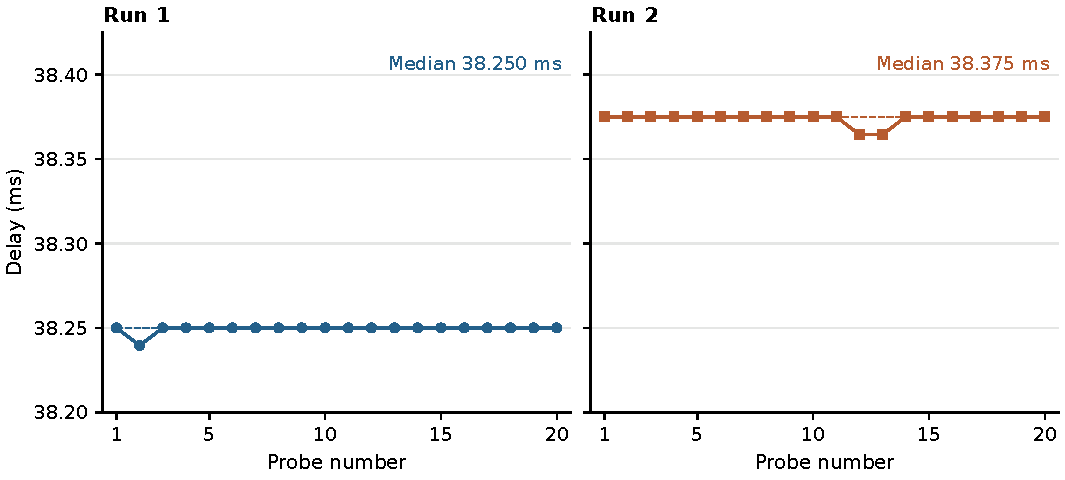
\includegraphics[width=\linewidth]{TimingSummary.pdf}
\par\vspace{3pt}
{\small\color{muted}Ranges: Run 1, 38.2396--38.2500\,ms; Run 2, 38.3646--38.3750\,ms. Each run's peak-to-peak spread was one sample (0.0104\,ms). Probes were 100\,Hz--20\,kHz sweeps.}

\vspace{13pt}
\textbf{Description.} The run medians differed by 0.125\,ms. Sample SD describes variation within each run's 20 quantized waveform estimates. These application roundtrip measurements include buffering and the acoustic path; the SD values do not establish calibrated timing accuracy.

\newpage
\topline
\pagetitle{Recorded frequency levels}{SONIC tone reconstruction\enspace$\cdot$\enspace14 frequencies\enspace$\cdot$\enspace2--27\,kHz}

\metrics{Tone duration}{10 ms}{Ramp duration}{2 ms}{Recorded pips}{16,800}

Locally reconstructed Sheep E tones in two 84-second blocks.

\vspace{3pt}
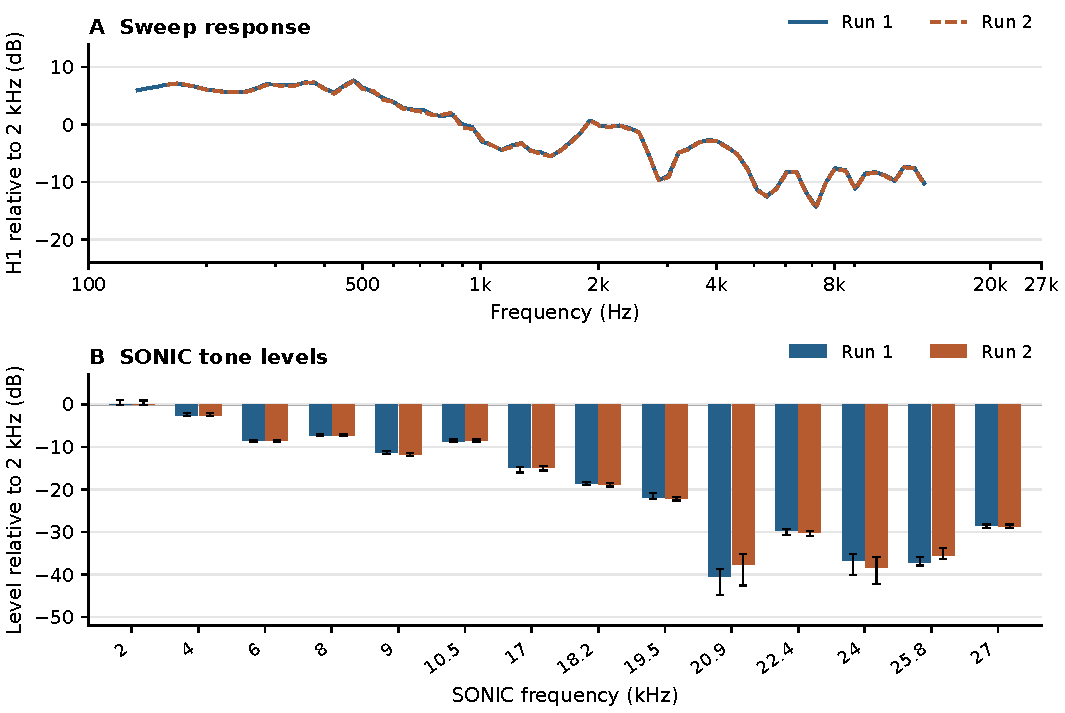
\includegraphics[width=\linewidth]{FrequencyResponse.pdf}
\par\vspace{2pt}
{\small\color{muted}Gaps mark unsupported sweep bands. Tone bars show medians; whiskers are 5th--95th percentiles of 600 pips per frequency per recording, not confidence intervals.}

\vspace{10pt}
\textbf{Description.} All 14 components appear in both recordings at unequal levels. Relative to 2\,kHz, 17--19.5\,kHz was 15--22\,dB lower; 20.9--25.8\,kHz was 30--40\,dB lower. These uncorrected full-chain measurements leave SPL, speaker-only response and distortion unqualified.

\textbf{Next.} Fix the geometry, calibrate microphone/SPL, test separated tones, and validate timing with an independent electrical reference.
\end{document}
